\documentclass{beamer}

\usetheme{default}
\beamertemplatenavigationsymbolsempty

%http://mikedewar.wordpress.com/2009/02/25/latex-beamer-python-beauty/
\definecolor{fore}{RGB}{249,242,215}
%{249,242,215}
\definecolor{back}{RGB}{51,51,51}
%{R\include{esa_python_block08_fileIO}GB}{51,51,51}
\definecolor{title}{RGB}{230,96,6}
%{255,0,90}
%http://meyerweb.com/eric/tools/color-blend/
%http://www.census.gov/population/international/data/worldpop/table_population.php
\setbeamercolor{titlelike}{fg=title}
\setbeamercolor{normal text}{fg=fore,bg=back}

\useinnertheme{rectangles}
\definecolor{UniBlue}{RGB}{34,139,34}
\setbeamercolor*{item}{fg=UniBlue}

\usepackage{colortbl}
\usepackage{caption}
\usepackage{listings,bera}
\usepackage{lipsum}
\newcommand\Fontvi{\fontsize{6}{6}\selectfont}
\newcommand\Fontvii{\fontsize{7}{7.5}\selectfont}
\newcommand\Fontviii{\fontsize{8}{9}\selectfont}
\newcommand\Fontix{\fontsize{9}{8.3}\selectfont}
\definecolor{keywords}{RGB}{255,102,0}
%{255,0,90}
\definecolor{comments}{RGB}{51,153,204}
%\definecolor{comments}{RGB}{83,121,170}
\setbeamertemplate{caption}[numbered]
%\useoutertheme{infolines}
\lstset{language=Python,
keywordstyle=\color{keywords},
commentstyle=\color{comments}\emph}

%\logo{epa-logo-full.jpg}

%example table
%\begin{frame}[fragile]
%\frametitle{Basic math operations}
%\begin{center}
%\begin{tabular}{lc} \hline
%\rowcolor{UniBlue!100}col1 & col2 \\ \hline \hline
%\rowcolor{UniBlue!75}3 & 3 \\ \hline
%\rowcolor{UniBlue!90}3 & 3 \\ \hline
%\rowcolor{UniBlue!75}3 & 3 \\ \hline
%\rowcolor{UniBlue!90}3 & 3 \\ \hline
%\end{tabular}
%\end{center}

% items enclosed in square brackets are optional; explanation below
\title[Title1]{Object-Oriented Programming}
\subtitle[Title2]{Python for Ecologists}
\author[etal]{Chance Pascale, Tom Purucker, Tao Hong}
\institute[EPA]{
  Ecological Society of America Workshop\\
  Portland, OR\\[1ex]
  \texttt{chancebatwalrus@gmail.com}
}

\begin{document}

%--- the titlepage frame -------------------------%
\begin{frame}[plain]
  \titlepage
\end{frame}

%\begin{frame}
%\frametitle{Frame with reduced font size}
%\Fontvi
%\lipsum[1]
%\end{frame}

%\begin{frame}
%\frametitle{Frame with regular font size}
%\lipsum[1]
%\end{frame}

%\begin{frame}[fragile]
%\frametitle{Generic slide}
%\begin{itemize}
%\item thing 1  
%\item thing 2 
%\item thing 3 
%\item thing 4
%\end{itemize} 
%\end{frame}

\begin{frame}[fragile]
\frametitle{Principles of OOP}
\begin{itemize}
  \item Classes
  \begin{itemize}
  \item Inheritance
  \item Abstraction 
  \item Encapsulation
  \item Polymorphism
\end{itemize}
  \item Methods
  \item Decoupling
\end{itemize} 
\end{frame}

\begin{frame}[fragile]
\frametitle{Let's take a gamble on classes}
\begin{itemize}
\item Fundamental data unit for card games is Card
\item Collection of Cards is Deck
\item Subset of the Deck is Hand
\item You need a CardGame to do something with the Cards, Deck, and Hands
\item OldMaidGame is an type of CardGame
\item OldMaidHand is a type of Hand used in OldMaidGame
\end{itemize} 
\end{frame}

\begin{frame}[fragile]
\frametitle{ULM a nice city in Germany, oops UML}
\begin{figure}
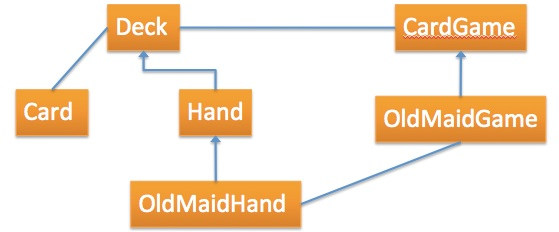
\includegraphics[scale=0.45]{ulm_uml.jpg} 
\caption{UML of OldMaidGame}
\end{figure}
\end{frame}

\begin{frame}[fragile]
\frametitle{Card Class Design}
\begin{itemize}
\item Each card has a suit and a value
\item Suits have no intrinsic use outside of a card so no real need to create a class for them
\item Values are sometimes integers and other times strings, so represent them as string and associate true value for each game
\end{itemize} 
\end{frame}

\begin{frame}[fragile]
\frametitle{Card Class Code}
\Fontviii
\begin{lstlisting}
class Card:
  suitList=["Clubs", "Diamonds", "Hearts", "Spades"]
  rankList=['Ace','2','3','4','5','6','7','8','9','10','Jack','Queen','King']

  def __init__(self, suit = 0, rank = 2):
    self.suit = suit
    self.rank = rank

  def __str__(self):
    return (self.rankList[self.rank] + " of " + self.suitList[self.suit])

  def __cmp__(self, other):
	if self.suit > other.suit: return 1
    if self.suit < other.suit: return -1
	if self.rank > other.rank: return 1
    if self.rank < other.rank: return -1
	return 0
\end{lstlisting}
\end{frame}

\begin{frame}[fragile]
\frametitle{Deck class design}
\begin{itemize}
\item A Deck is a collection of cards
\item General functionality of decks are that they can be shuffled, the 'top' card can be drawn, and many times knowing if there are any cards in the deck is necessary 
\end{itemize} 
\end{frame}

\begin{frame}[fragile]
\frametitle{Deck Class Code}
\begin{lstlisting}
class Deck:
  def __init__(self):
    self.cards = []
    for suit in range(4):
      for rank in range(1, 14):
        self.cards.append(Card(suit, rank))

  def printDeck(self):
    for card in self.cards:
      print card 

  def __str__(self):
    s = ""
    for i in range(len(self.cards)):
      s = s + " " * i + str(self.cards[i]) + "\n"
    return s

\end{lstlisting}
\end{frame}

\begin{frame}[fragile]
\frametitle{Deck Class Code (continued)}
\fontvi
\begin{lstlisting}
  def shuffle(self):
    import random
    nCards = len(self.cards)
    for i in range(nCards):
      j = random.randrange(i, nCards)
      self.cards[i],self.cards[j]=
           self.cards[j],self.cards[i]
  def removeCard(self, card):
    if card in self.cards:
      self.cards.remove(card)
      return True
    else:
      return False
  def popCard(self):
    return self.cards.pop()
  def isEmpty(self):
    return (len(self.cards) == 0)
\end{lstlisting}
\end{frame}

\begin{frame}[fragile]
\frametitle{Hand Class Design}
\begin{itemize}
\item Hand is an example of a Deck, a subset of the complete deck
\item If we make Hand inherit from Deck, then we get the data structures that Deck contains
\item Hand can also call the methods of Deck as if it was the superclass
\item If a method of Deck class is not included in Hand code, then if that method is called on Hand object Deck method will be used.
\end{itemize} 
\end{frame}

\begin{frame}[fragile]
\frametitle{Hand Class Code}
\fontvi
\begin{lstlisting}
class Hand(Deck):
  pass
  def __init__(self, name = ""):
    self.cards = []
    self.name = name

  def addCard(self, card):
    self.cards.append(card)

  def deal(self, hands, nCards = 999):
    nHands = len(hands)
      for i in range(nCards):
        if self.isEmpty():
          break # break if out of cards
        card = self.popCard() # take the top card
        hand = hands[i % nHands] # whose turn is next?
        hand.addCard(card) # add the card to the hand
\end{lstlisting}
\end{frame}

\begin{frame}[fragile]
\frametitle{Hand Class Code (continued)}
\fontvi
\begin{lstlisting}
# if next function not in code 
# Deck __str__ would be called
  def __str__(self):
    s = "Hand " + self.name
    if self.isEmpty():
      return s + " is empty\n"
    else:
      return s + " contains\n" + Deck.__str__(self)
\end{lstlisting}
\end{frame}

\begin{frame}[fragile]
\frametitle{CardGame Class Design/Code}
\fontvi
\begin{itemize}
\item Card games contain a single deck, which should be shuffled at the beginning of each game
\end{itemize}
\begin{lstlisting}
class CardGame:

  def __init__(self):
    self.deck = Deck()
    self.deck.shuffle()
\end{lstlisting}
\end{frame}

\begin{frame}[fragile]
\frametitle{OldMaidHand Design/Code}
\fontvi
\begin{itemize}
\item Pretty much a normal card hand but needs method to find and remove all matches and return a count of matches
\end{itemize}
\begin{lstlisting}
class OldMaidHand(Hand):
  def removeMatches(self):
    count = 0
    originalCards = self.cards[:]
    for card in originalCards:
      match = Card(3 - card.suit, card.rank)
      if match in self.cards:
        self.cards.remove(card)
        self.cards.remove(match)
        print "Hand %s: %s matches %s" % 
             (self.name, card, match)
        count = count + 1
      return count

\end{lstlisting}
\end{frame}

\begin{frame}[fragile]
\frametitle{OldMaidGame Design}
\begin{itemize}
\item Like all classes that 'extend' CardGame, a deck is needed and it should be shuffled, oh wait CardGame already does this
\item Playing the game performs the following steps:
\begin{enumerate}
\item Take the Queen of hearts out of the deck
\item Deal OldMaidHands
\item Remove and count number of matches
\item Each turn for a player is the same(25 turns):
\begin{enumerate}
\item Check if hand is empty, if so do nothing
\item Take neighbor player’s “top” card
\item Remove and count number of matches
\item Shuffle your hand
\end{enumerate}
\item Top score after all turns is winner
\end{enumerate}
\end{itemize} 
\end{frame}

\begin{frame}[fragile]
\frametitle{OldMaidGame Code}
\Fontix
\begin{lstlisting}
class OldMaidGame(CardGame):
    def play(self, names):
        self.deck.removeCard(Card(0, 12)) # remove Queen of Clubs 
       self.hands = [] # make a hand for each player 
        for name in names :
            self.hands.append(OldMaidHand(name))
            # deal the cards 
            self.deck.deal(self.hands)
            print "---------- Cards have been dealt"
            self.printHands()
            # remove initial matches 
            matches = self.removeAllMatches()
            print "---------- Matches discarded, play begins"
            self.printHands()
	    turn = 0  # play until all 50 cards are matched 
        numHands = len(self.hands)
        while matches < 25:
            matches = matches + self.playOneTurn(turn)
            turn = (turn + 1) % numHands
            print "---------- Game is Over"
            self.printHands()
\end{lstlisting}
\end{frame}

\begin{frame}[fragile]
\frametitle{OldMaidGame Code (continued)}
\Fontix
\begin{lstlisting}
 def removeAllMatches(self):
        count = 0
        for hand in self.hands:
            count = count + hand.removeMatches()
        return count
   
 def playOneTurn(self, i):
        if self.hands[i].isEmpty():
            return 0
        neighbor = self.findNeighbor(i)
        pickedCard = self.hands[neighbor].popCard()
        self.hands[i].addCard(pickedCard)
        print "Hand", self.hands[i].name, "picked", pickedCard
        count = self.hands[i].removeMatches()
        self.hands[i].shuffle()
        return count
\end{lstlisting}
\end{frame}

\begin{frame}[fragile]
\frametitle{OldMaidGame Code (continued)}
\begin{lstlisting}
 def findNeighbor(self, i):
        numHands = len(self.hands)
        for next in range(1, numHands):
            neighbor = (i + next) % numHands
            if not self.hands[neighbor].isEmpty():
                return neighbor

\end{lstlisting}
\end{frame}

\begin{frame}[fragile]
\frametitle{What is \_\_init\_\_.py}
\begin{itemize}
\item Files named \_\_init\_\_.py are used to mark directories on disk as a Python package directories. If you have the files
\item mydir/spam/\_\_init\_\_.py mydir/spam/module.py and mydir is on your path, you can import the code in module.py as:
\item import spam.module or
\item from spam import module If you remove the \_\_init\_\_.py file, Python will no longer look for submodules inside that directory, so attempts to import the module will fail.
\item The \_\_init\_\_.py file is usually empty, but can be used to export selected portions of the package under more convenient names, hold convenience functions, etc. Given the example above, the contents of the \_\_init\_\_ module can be accessed as
\item import spam
\end{itemize} 
\end{frame}

\end{document}